%% 
%% Copyright 2007-2024 Elsevier Ltd
%% 
%% This file is part of the 'Elsarticle Bundle'.
%% ---------------------------------------------
%% 
%% It may be distributed under the conditions of the LaTeX Project Public
%% License, either version 1.3 of this license or (at your option) any
%% later version.  The latest version of this license is in
%%    http://www.latex-project.org/lppl.txt
%% and version 1.3 or later is part of all distributions of LaTeX
%% version 1999/12/01 or later.
%% 
%% The list of all files belonging to the 'Elsarticle Bundle' is
%% given in the file `manifest.txt'.
%% 
%% Template article for Elsevier's document class `elsarticle'
%% with numbered style bibliographic references
%% SP 2008/03/01
%% $Id: elsarticle-template-num.tex 249 2024-04-06 10:51:24Z rishi $
%%
\documentclass[preprint,12pt]{elsarticle}

%% Use the option review to obtain double line spacing
%% \documentclass[authoryear,preprint,review,12pt]{elsarticle}

%% Use the options 1p,twocolumn; 3p; 3p,twocolumn; 5p; or 5p,twocolumn
%% for a journal layout:
%% \documentclass[final,1p,times]{elsarticle}
%% \documentclass[final,1p,times,twocolumn]{elsarticle}
%% \documentclass[final,3p,times]{elsarticle}
%% \documentclass[final,3p,times,twocolumn]{elsarticle}
%% \documentclass[final,5p,times]{elsarticle}
%% \documentclass[final,5p,times,twocolumn]{elsarticle}

%% For including figures, graphicx.sty has been loaded in
%% elsarticle.cls. If you prefer to use the old commands
%% please give \usepackage{epsfig}

%% The amssymb package provides various useful mathematical symbols
\usepackage{amssymb}
%% The amsmath package provides various useful equation environments.
\usepackage{amsmath}
%% The amsthm package provides extended theorem environments
%% \usepackage{amsthm}

%% The lineno packages adds line numbers. Start line numbering with
%% \begin{linenumbers}, end it with \end{linenumbers}. Or switch it on
%% for the whole article with \linenumbers.
%% \usepackage{lineno}

\journal{Fusion Engineering and Design}

\begin{document}

\begin{frontmatter}

%% Title, authors and addresses

%% use the tnoteref command within \title for footnotes;
%% use the tnotetext command for theassociated footnote;
%% use the fnref command within \author or \affiliation for footnotes;
%% use the fntext command for theassociated footnote;
%% use the corref command within \author for corresponding author footnotes;
%% use the cortext command for theassociated footnote;
%% use the ead command for the email address,
%% and the form \ead[url] for the home page:
%% \title{Title\tnoteref{label1}}
%% \tnotetext[label1]{}
%% \author{Name\corref{cor1}\fnref{label2}}
%% \ead{email address}
%% \ead[url]{home page}
%% \fntext[label2]{}
%% \cortext[cor1]{}
%% \affiliation{organization={},
%%             addressline={},
%%             city={},
%%             postcode={},
%%             state={},
%%             country={}}
%% \fntext[label3]{}

\title{JET Plasma Control System Upgrade using MARTe2}

%% use optional labels to link authors explicitly to addresses:
%% \author[label1,label2]{}
%% \affiliation[label1]{organization={},
%%             addressline={},
%%             city={},
%%             postcode={},
%%             state={},
%%             country={}}
%%
%% \affiliation[label2]{organization={},
%%             addressline={},
%%             city={},
%%             postcode={},
%%             state={},
%%             country={}}

\author{A.V.~Stephen} %% Author name

%% Author affiliation
\affiliation{organization={Computing Division, United Kingdom Atomic Energy Authority},%Department and Organization
            addressline={Culham Campus}, 
            city={Abingdon},
            postcode={OX14 3DB}, 
            state={Oxfordshire},
            country={United Kingdom}}

%% Abstract
\begin{abstract}
%% Text of abstract

JET real-time plasma control has been delivered with a heterogeneous collection of control systems linked by a dedicated low-jitter, low-latency network. To provide a high degree of flexibility in tuning plasma control algorithms to experimental requirements, the Real-Time Central Controller (RTCC) has been available since 1997. RTCC provides a sandboxed execution environment where experimental algorithms can be deployed with a rapid development workflow. New control laws can be developed by operators during the course of an experimental session. The potential impact of a defect in algorithms evolved without full lifecycle quality assurance can be bounded by clipping feedback control requests at the actuator managers. The likelihood of such defects is reduced in the first place by constraining the algorithms to be composed from reusable blocks and trusted real-time signals. Although this system operated successfully for a long time, limitations in compute capacity of the legacy hardware on which the application was deployed constrained algorithm development.

Motivated by the need to provide physics operators with a more performant system, an upgrade project was carried out to port the RTCC application to a modern high performance PC platform. The architecture selected was to use the MARTe2 framework. Development was able to reuse existing MARTe2 data sources to connect the application to the JET environment using the ITER SDN protocol. RTCC blocks were converted to MARTe2 functions. Python tooling was created to automatically convert previously deployed RTCC algorithms to MARTe2 configuration form.

This paper describes the techniques used to demonstrate system correctness prior to deployment in the JET operating environment. This was particularly important given that it was deployed around the time of the DT campaigns. It explains how the system was used to demonstrate some novel control methods which delivered useful experiments in the final JET campaigns. It also outlines how the JET legacy data combined with this MARTe2 application can offer future value, even in the absence of the JET machine itself.
\end{abstract}

%%Graphical abstract
%% TODO: This is recommended
%\begin{graphicalabstract}
%\includegraphics{grabs}
%\end{graphicalabstract}

%% TODO: This is recommended
%%Research highlights
%%\begin{highlights}
%\item Research highlight 1
%\item Research highlight 2
%\end{highlights}

%% Keywords
\begin{keyword}
%% keywords here, in the form: keyword \sep keyword
real-time \sep control \sep MARTe2 \sep JET \sep QA

%% PACS codes here, in the form: \PACS code \sep code

%% MSC codes here, in the form: \MSC code \sep code
%% or \MSC[2008] code \sep code (2000 is the default)

\end{keyword}

\end{frontmatter}

%% Add \usepackage{lineno} before \begin{document} and uncomment 
%% following line to enable line numbers
%% \linenumbers

%% main text
%%

%% Use \section commands to start a section
\section{Introduction}
\label{sec:intro}
%% Labels are used to cross-reference an item using \ref command.

\subsection{Background}

Plasma Control Systems\footnote{PCS - Plasma Control System} are large and complex.
There are variations in approach, but most fusion projects distinguish between
the disciplines of algorithm design and real-time system implementation.
The former abstracts higher level descriptions of the plasma control processes
from the physics perspective. Thus dealing with magnetic, kinetic, MHD and error field
control as well as wall conditioning, disruption and runaway electron control.
Real-time system implementation must then map the control tasks into robust, resilient,
deterministic control software. The implementation must deal with practical real-world
constraints. These include signal processing to compute the required algorithm
inputs, management of target control references throughout the shot, and provision 
of exceptional handling strategies to resolve off-normal conditions (whether in the plasma,
or in the sensor and actuator subsystems).

% TODO\cite
% https://www.sciencedirect.com/science/article/abs/pii/S0920379614000647
% Physics of the conceptual design of the ITER plasma control system 
%
%
% NO IT DOESN'T : IT DESCRIBES ONE UPGRADE WHICH TACKLED BOTH-ish

This paper concentrates on the second challenge, of real-time plasma control system implementation.

The order of the paper is $\ldots$ % TODO



% RENAME Materials and Methods, but that is the spirit
\section{Architecture and Infrastructure}

\subsection{JET PCS Architecture}

The JET PCS architecture was
{\em distributed} and {\em heterogeneous}\footnote{JET has entered decommissioning, and although the PCS systems still exist, they no longer operate}.  
The design choice to separate it into around 80 subsystems supported broad delegation of responsibility and
promoted maximal separation of concerns. This proved to be beneficial as the project lifetime was repeatedly extended and as the machine configuration was 
significantly upgraded.  The heterogeneous hardware and software components selected for implementation were partly imposed by necessity as the project outlived successive generations of vendor supported  technology and partly by differences in requirements for individual subsystems.

\begin{figure}[t]%% placement specifier
%% Use \includegraphics command to insert graphic files. Place graphics files in 
%% working directory.
\centering%% For centre alignment of image.
%\includegraphics{example-image-a}
	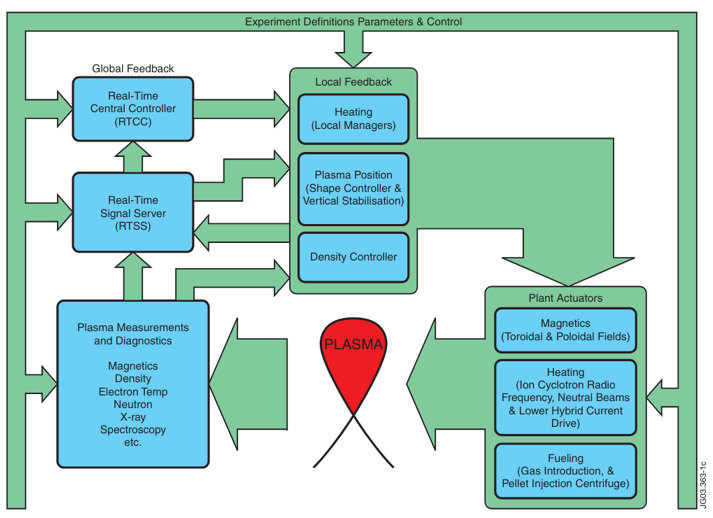
\includegraphics{JG_Felton}
\vspace{1.5in}
%% Use \caption command for figure caption and label.
\caption{Figure Caption}\label{fig1}
%% https://en.wikibooks.org/wiki/LaTeX/Importing_Graphics#Importing_external_graphics
\end{figure}

\subsection{Primary Feedback Control Loops}

\label{s_primary_fb}

The primary feedback control loops can be seen as independent subsets of the overall JET PCS
comprising sensor, state estimation and actuator control functions.

\begin{enumerate}
	\item{Magnetic sensors and the Plasma Current, Shape and Vertical Control}
	\item{Density instrumentation, validation and gas feedback control.}
	\item{Neutral-beam power injection control to achieve fixed reference.}
	\item{Radio frequency power injection control to achieve fixed ion heating.}
\end{enumerate}

\subsection{JET Real-time Central Controller}
\label{s_rtcc}

As described in \ref{s_primary_fb} the primary basic control were
engineered as separate subsystems comprising broadly fixed algorithms
for sensor signal processing, state estimation and feedback control.
These had primary responsibility for establishing plasmas of an
appropriate type to meet scientific task force baseline scenarios.

To provide more advanced control, of plasma parameters for which the
relationship between direct measurement and fixed actuator response, 
it was necessary to add a more flexible and dynamic controller.

Termed the {\em real-time central controller (RTCC)} this system was
part of a suite of general real-time services targeting advanced
real-time control research.  The RTCC system was an application 
capable of receiving a very wide (and variable) set of input signals
aggregated and managed by a companion system, the {\em real-time signal server (RTSS)}.

The architecture of this RTCC application was the common pattern of
a real-time execution engine configurable with a graph of signal
processing blocks.  The library of blocks supported signal ingress,
filtering and validation to achieve estimates of plasma parameter
state.  Entities to implement control schemes, such as a proportional/integral/derivative
(PID controller), transfer functions and general calculation support
could then be combined to explore control concepts.  An option to
use real-time computed references for the actuator systems, and to 
use these in place of the nominal feedfoward time series was also
provided.

Software tools for control room staff provided an environment with
which to prepare new control concepts which could be used during operations
without a lengthy software validation and commissioning process.
The justifications for permitting this were numerous architectural
features and operational procedures which reduced the risk that a 
serious mis-control of the machine might occur.

The algorithm definitions, termed {\em RTCC networks}, formed a corpus
of executable, reusable research results in the area of plasma control.

The same architecture, but implemented with independent hardware
and an independent configuration management system and procedure 
was adopted as part of the project to protect the ITER-like wall
(PIW project) in 2011.

\subsubsection{RTCC Drivers for Upgrade}

Infrastructure weaknesses $\ldots$

Making the case for an upgrade to the RTCC system was organisationally
challenging, in spite of the recognised technical limitations of the system.
These included restrictions on the size and complexity of RTCC networks
as well as the need for specialist training to become competent in
using the system and re-engineering previously developed networks.

\subsubsection{Requirements and Contraints}


\begin{enumerate}
	\item{Backwards compatibility}
	\item{Increased capacity}
	\item{Minimise risk to operations}
	\item{Support new components (blocks)}
	\item{Improve physics user experience}
	\item{Enhance JET legacy (code and data)}
\end{enumerate}

\section{Methodology and Design Approach}

% FIGURE? JG03.363-1c ? The Felton diagram.

%% TOCITE Level-1 paper ?

Overall coordination and configuration of these disparate systems was achieved through coordinating systems, services
and applications.

\subsection{JET Software Design Principles}

Engineers across the JET project recognised the need to structure applications to be highly data driven.
This was achieved from early in the project in the architecture of the {\em drivers} and {\em general acquisition program (gap)} applications.
These abstracted the representation of the electronics channels (drivers) and the signals to be acquired (gap) 
from the details of the operating system.  New hardware was added by inserting additional records into 
the drivers configuration database.  New, or modified signal collection definitions
were created by updating the gap configuration database.  In both cases, objects in the 
configuration databases implemented common behaviours relevant to the application requirements.
A note of historical interest is that these applications were completed in the late 1980s
but architecturally were extremely similar to the EPICS system whioch was first released in 1994.
%\cite EPICS

\subsection{Software Frameworks}

The JET CODAS diagnostics integration team designed a component oriented framework (CFW)
for rapid application development. The design style was object oriented, though
written in C due to legacy constraints.  At the core of the design was the concept
that an application be described through a structured configuration file.
The configuration file used a declarative language to compose an application
from component instances. Each component provided a set of modifiable attributes.
Attribute values could be constants (scalar, or user defined types) or 
references to other components.  The target use case for this framework was supervisory
control applications implementing monitoring and control, but operating 24x7 and 
tasked with slow, asynchronous operations.

In addition to defining the CFW declarative language, a broader descriptive language
called CODAS Configuration Language (CCL) was designed in parallel.  This was motivated 
to provide an efficient tool with which to create CFW "programs".  The observation
was that as application complexity scales, a declarative component based system
requires the powers of abstraction common to most general programming languages.
i.e. It is desirable to be able to express iteration, conditional existence, 
and algorithmically described variability.  Support for text manipulation is
beneficial to be able to create human comprehensible names.

A formal approach to describing the CCL system was taken, including use of W3C
standards for managing namespaces and vocabularies, and making the declarative
form compatible with RDF (resource data framework).

Contemporaneously with this CFW development, the Plasma Operations Group had decided
to take a very structurally equivalent approach to building real-time control applications.
Their application, the now well known Multi-threaded Application for Real-Time execution (MARTe),
also consists in a run-time which instantiates objects from a structured configuration file.
Implemented in C++, and targeting high performance, low jitter, high reliability control
applications it also provided some measure of tooling for rapid application development.
To manage the aggregation and customisation of configuration files, MARTe at JET made
use of the Level-1 configuration tool to manage templates, parameter substitution and
code generation algorithms.

JET plasma control made significant use of the MARTe system, implementing key systems
including shape control, vertical stabilisation, walls (estimating the energy load on the first wall),
EFCC control, vessel-thermal map and the ILW real-time protection sequencer.  These applications
were in use from the early 2000s and were fully integrated with the other JET operations software
(configuration, monitoring, data acquisition and the RTDN ATM network).

Around 2014, at F4E, following failed attempts to find a comparable COTS software system 
on the market, a project to harden MARTe to a level suitable for deployment at ITER 
was undertaken.  The outcome of this work was MARTe2.  In addition to code review and improvement,


\subsection{Real-Time Data Network}

The second unifying service was the real-time data network. This was a high performance, dedicated private network with low latency and low jitter communications between all of the PCS systems.  The communications topology was point to multi-point. Implementation translated across three generations of networking equipment.  The early version of the network ran over 100Mbps ethernet using UDP unicast. An upgrade in the mid 1990s introduced telecommunication standard equipment using ATM\footnote{} switches in which the delivery of data was configured in the switch. In 2016, motivated by the increasing difficulty in obtaining ATM equipment, the ITER SDN ethernet multicast solution was adopted.

\subsection{Configuration Management}

  Most importantly, the {\em Level-1} configuration management subsystem provided a consistent and detailed model of each subsystem. Representing the attributes and modifiable options for each subsystem as rich parameters, the {\em Level-1} database, user interfaces, and codes provided a meta-programming system for the overall PCS.  This configuration tooling was
used to define all of the control settings to achieve a given experimental goal (parameter values, calibration, reference time series and inter-system dependencies).  This system tuning was required to be completed before a JET discharge could begin.  

 

\subsubsection{Upgrade Plan}

Making the case for an upgrade to the RTCC system was organisationally
challenging, in spite of the recognised technical limitations of the system.
These included restrictions on the size and complexity of RTCC networks
as well as the need for specialist training to become competent in
using the system and re-engineering previously developed networks.



\section{Upgrade Outcomes and Benefits}

Each of the calculation blocks in the RTCC application were ported to MARTe2 {\em Functions}.
Atypically, the standard block template consisted in a combined vector of value and status.
This protocol was retained in the updated implementation. This was important to simplify
translating algorithm definitions from the original notation to MARTe2 format.

The outline structure of the RTCC2 MARTe2 application was istraightforward.
High level service declarations common to most JET MARTe applications
instantiated an introspection service, a pulse oriented state machine, 
and the main data flow superstructure.

Python translation support modules handled the translation of RTCC network 
descriptions into MARTe2 configuration syntax, using the new {\em Functions}.
In addition to generating the {\em Function} instances (a simple 1:1 mapping),
the translation also created auxiliary objects to manage automatic
recording of computed values.  Managing automatic name generation is one
of the main tasks in this process.  This introduces a design question.  From
the perspective of efficiency, and to simplify the translation code, 
auto-generated names which lack comprehensibility are a good choice. 
This leaves code review in the domain of the meta-programming code, 
which is practical for checking the intent.  The disadvantage of this
approach however is that if the detailed results from executing the 
algorithms differ from expected values, it is difficult to analyse
the intermediate signals as their relationship to the calculation is
masked by the anonymous names.


\section{Discussion}

Granularity, reuse and code generation.

The question of how to preserve human readability of generated code...

\subsection{Engineering Approaches}

\begin{itemize}
\item{Monolithic}
\item{Distributed}
\item{MBSE}
\item{Custom Code}
\item{Frameworks}
\item{Integration Ecosystems}
\end{itemize}

\subsubsection{Domain Specific Languages (DSLs)}

Where data driven applications achieve a certain level of reconfiguration, they are more commonly
described in computer science as {\em domain specific languages (DSLs)}. DSLs are characterised
as a programming language designed for a specific use case.  Benefits of DSLs are that they 
offer a higher level of abstraction optimized for a specific class of problem. Two classes
of domain specific language are typically identified. {\em External} DSLs separate the DSL
code from the standard code (written in a general programming language).  {\em Internal} DSLs
mix the DSL code and the general-purpose code in the same file.  This is general achieved by
embedding the DSL into the general-purpose code as a set of libraries or extensions.

In both cases, there is a challenge to adequately support the new task of programming
in the invented language.  To be effective, general purpose programming languages must
formally define syntax and semantics. They must be supplied with compilers, or interpreters.
These language tools are expected to be extended with support for trapping and explaining
syntax errors as a minimum, and semantic errors preferably.  To increase productivity, 
engineers working in a language also expect more advanced features such as code completion
and automated documentation.

For external DSLs, providing language support for basic control flow and iteration
can help to make programs more efficient and comprehensible.  A common design pattern
to deliver this support is to use code templating and code generation.  This
{\em meta-programming} increases productivity, but at the cost of adding another
layer of complexity in the tool stack.


\

\section{Conclusion}

% Comments on DSLs and tooling.


\section{Glossary}

Field specific terms.

\begin{itemize}
\item[ATM]{Asynchronous Transmission Mode.  A low-latency telecommunications protocol standard.}
\item[DSL]{Domain Specific Language}
\item[MARTe]{Multi-threaded Application for Real-Time execution.  Software framework from JET.}
\item[MARTe2]{Enhanced version of MARTe developed by F4E for ITER.}
\item[Real-Time Thread]{The unit of concurrency in a MARTe2 application.}
\item[DataSource]{A service which abstracts device drivers to handle application I/O in a MARTe2 application.}
\item[Function]{The unit of compute in a MARTe2 application.  Each Real-Time Thread calls one or more Functions.}
\item[JET]{Joint European Tokamak}
\item[MBSE]{Model Based System Engineering}
\item[PCS]{Plasma Control System}
\item[RTCC]{Real-Time Central Controller.  A core application in the JET PCS.}
\item[SDN]{Synchronous Databus Network.  An ITER real-time network protocol.}
\item[UDP]{User Datagram Protocol. A connectionless data transport method in networking.}
\end{itemize}

\section{Abbreviations}

Check that non-standard abbrevs are defined in a footnote on page 1.

\section{Acknowledgements}

Individuals who helped (but were not co-authors).

\section{Author Contributions}
Using CRediT taxonomy.

\begin{itemize}
\item[Conceptualization]{}
\item[Data Curation]{}
\item[Formal analysis ]{}
\item[Funding acquisition]{}
\item[Investigation]{}
\item[Methodology]{}
\item[Project administration]{}
\item[Resources]{}
\item[Software]{}
\item[Supervision]{}
\item[Validation]{}
\item[Visualization]{}
\item[Writing - draft]{}
\item[Writing - review and editing]{}
%% See https://www.elsevier.com/researcher/author/policies-and-guidelines/credit-author-statement
\end{itemize}

\section{Funding}

This work was supported by $ldots$
%% The Appendices part is started with the command \appendix;
%% appendix sections are then done as normal sections

\appendix
\section{Example Appendix Section}
\label{app1}

Appendix text.

%% For citations use: 
%%       \cite{<label>} ==> [1]

%%
Example citation, See \cite{lamport94}.

%% If you have bib database file and want bibtex to generate the
%% bibitems, please use
%%
%%  \bibliographystyle{elsarticle-num} 
%%  \bibliography{<your bibdatabase>}

%% else use the following coding to input the bibitems directly in the
%% TeX file.

%% Refer following link for more details about bibliography and citations.
%% https://en.wikibooks.org/wiki/LaTeX/Bibliography_Management

\begin{thebibliography}{00}

%% For numbered reference style
%% \bibitem{label}
%% Text of bibliographic item

\bibitem{lamport94}
  Leslie Lamport,
  \textit{\LaTeX: a document preparation system},
  Addison Wesley, Massachusetts,
  2nd edition,
  1994.

\end{thebibliography}
\end{document}

\endinput
%
%% Template Code follows


%% Use \subsection commands to start a subsection.
\subsection{Example Subsection}
\label{subsec1}

Subsection text.

%% Use \subsubsection, \paragraph, \subparagraph commands to 
%% start 3rd, 4th and 5th level sections.
%% Refer following link for more details.
%% https://en.wikibooks.org/wiki/LaTeX/Document_Structure#Sectioning_commands

\subsubsection{Mathematics}
%% Inline mathematics is tagged between $ symbols.
This is an example for the symbol $\alpha$ tagged as inline mathematics.

%% Displayed equations can be tagged using various environments. 
%% Single line equations can be tagged using the equation environment.
\begin{equation}
f(x) = (x+a)(x+b)
\end{equation}

%% Unnumbered equations are tagged using starred versions of the environment.
%% amsmath package needs to be loaded for the starred version of equation environment.
\begin{equation*}
f(x) = (x+a)(x+b)
\end{equation*}

%% align or eqnarray environments can be used for multi line equations.
%% & is used to mark alignment points in equations.
%% \\ is used to end a row in a multiline equation.
\begin{align}
 f(x) &= (x+a)(x+b) \\
      &= x^2 + (a+b)x + ab
\end{align}

\begin{eqnarray}
 f(x) &=& (x+a)(x+b) \nonumber\\ %% If equation numbering is not needed for a row use \nonumber.
      &=& x^2 + (a+b)x + ab
\end{eqnarray}

%% Unnumbered versions of align and eqnarray
\begin{align*}
 f(x) &= (x+a)(x+b) \\
      &= x^2 + (a+b)x + ab
\end{align*}

\begin{eqnarray*}
 f(x)&=& (x+a)(x+b) \\
     &=& x^2 + (a+b)x + ab
\end{eqnarray*}

%% Refer following link for more details.
%% https://en.wikibooks.org/wiki/LaTeX/Mathematics
%% https://en.wikibooks.org/wiki/LaTeX/Advanced_Mathematics

%% Use a table environment to create tables.
%% Refer following link for more details.
%% https://en.wikibooks.org/wiki/LaTeX/Tables
\begin{table}[t]%% placement specifier
%% Use tabular environment to tag the tabular data.
%% https://en.wikibooks.org/wiki/LaTeX/Tables#The_tabular_environment
\centering%% For centre alignment of tabular.
\begin{tabular}{l c r}%% Table column specifiers
%% Tabular cells are separated by &
  1 & 2 & 3 \\ %% A tabular row ends with \\
  4 & 5 & 6 \\
  7 & 8 & 9 \\
\end{tabular}
%% Use \caption command for table caption and label.
\caption{Table Caption}\label{fig1}
\end{table}


%% Use figure environment to create figures
%% Refer following link for more details.
%% https://en.wikibooks.org/wiki/LaTeX/Floats,_Figures_and_Captions
\begin{figure}[t]%% placement specifier
%% Use \includegraphics command to insert graphic files. Place graphics files in 
%% working directory.
\centering%% For centre alignment of image.
\includegraphics{example-image-a}
%% Use \caption command for figure caption and label.
\caption{Figure Caption}\label{fig1}
%% https://en.wikibooks.org/wiki/LaTeX/Importing_Graphics#Importing_external_graphics
\end{figure}


%% The Appendices part is started with the command \appendix;
%% appendix sections are then done as normal sections
\appendix
\section{Example Appendix Section}
\label{app1}

Appendix text.

%% For citations use: 
%%       \cite{<label>} ==> [1]

%%
Example citation, See \cite{lamport94}.

%% If you have bib database file and want bibtex to generate the
%% bibitems, please use
%%
%%  \bibliographystyle{elsarticle-num} 
%%  \bibliography{<your bibdatabase>}

%% else use the following coding to input the bibitems directly in the
%% TeX file.

%% Refer following link for more details about bibliography and citations.
%% https://en.wikibooks.org/wiki/LaTeX/Bibliography_Management

\begin{thebibliography}{00}

%% For numbered reference style
%% \bibitem{label}
%% Text of bibliographic item

\bibitem{lamport94}
  Leslie Lamport,
  \textit{\LaTeX: a document preparation system},
  Addison Wesley, Massachusetts,
  2nd edition,
  1994.

\end{thebibliography}
\end{document}

\endinput
%%
%% End of file `elsarticle-template-num.tex'.

